\documentclass[a4paper,10pt]{article}

\usepackage{graphicx}
\usepackage{amsmath}
\usepackage{mathtools}
\usepackage[spanish]{babel}
\usepackage[utf8]{inputenc} % Permite escribir directamente áéíóúñ
\usepackage{float}
\usepackage[hidelinks]{hyperref}
\usepackage{pdfpages}
\usepackage{multirow}
\usepackage[margin=0.9in]{geometry}

\title{ \textbf{ 7529. Teoría de Algoritmos I\\
Trabajo Práctico 2}}

\author{ Ferreyra, Oscar, \textit{Padrón Nro. 89563} \\
\texttt{ fferreyra38@gmail.com } \\[2.5ex]
Martin, Débora, \textit{Padrón Nro. 90934} \\
\texttt{ demartin@fi.uba.ar } \\[2.5ex]
Eisner, Ariel, \textit{Padrón Nro. 90697} \\
\texttt{ aeeisnerg@gmail.com } \\[2.5ex]
\normalsize{2do. Cuatrimestre de 2016} \\
}

\date{}

\begin{document}
\maketitle
\thispagestyle{empty} % quita el nro en la primer pagina
\setcounter{page}{0}
\newpage
\tableofcontents

\newpage

\section{Programación dinamica}


\subsection{El problema de la mochila}

Dado un conjunto de elementos S={1,2,{\dots}} el problema consiste encontrar la secuencia X=() que maximice:

\begin{equation*}
\displaystyle\sum_{i=1}^{10} t_i
\displaystyle\sum_{i=S}^{} v_ix_i
\end{equation*}

\bigskip

\textcolor[rgb]{0.06666667,0.06666667,0.06666667}{con la restricción:}

\begin{equation*}
\sum _{i = S}^{}w_ix_i<W
\end{equation*}

\bigskip

donde 
\begin{equation*}v_i, w_i, W \geq 0\end{equation*} y 
\begin{equation*} x_i \in \{0,1\}.\end{equation*}


\textbf{\textcolor{black}{Pruebas}}


\bigskip

{\centering
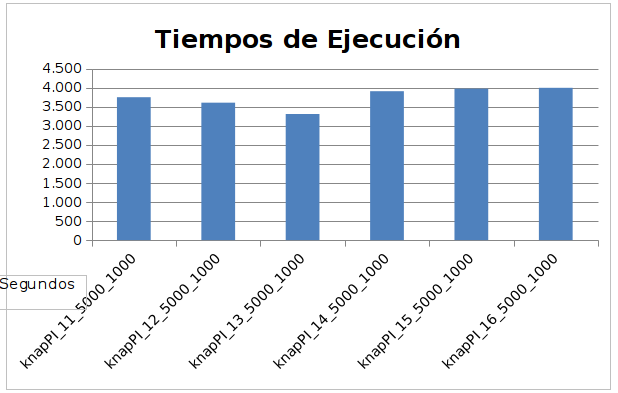
\includegraphics[width=11.589cm,height=7.482cm]{Tp27529-img003.png}
\par}


\bigskip

Se seleccionó el lote de archivos con sufijo 5000\_1000 del archivo \href{http://www.diku.dk/~pisinger/hardinstances_pisinger.tgz}{\textbf{\textcolor[rgb]{0.0,0.0,0.039215688}{hardinstances.tgz}}} dado que los demás archivos generaban matrices demasiado grandes y el programa abortaba por falta de memoria.

\bigskip
\bigskip


\subsection{El problema del viajante de comercio}
Al implementar el algoritmo de Bellman-Held-Karp se notó que insume una gran cantidad de espacio en memoria, por lo que no fue posible realizar corridas para matrices de orden superior. El espacio en memoria que insume este algoritmo es del orden de $O(2^n n)$.

La complejidad del algoritmo se calcula en $O(2^n n^2)$ debido a las comparaciones realizadas y la adición de elementos a los distintos sets. A continuación se muestran los tiempos de ejecución dependiendo de la cantidad de vertices.

\begin{table}[H]
\centering
\begin{tabular}{|c|c|c|c|c|c|c|}
\hline
Cantidad de ciudades	& Tiempo de ejecución (segundos)\\\hline
15						& 16\\\hline
17						& 299\\\hline
19						& 7237\\\hline
21						& 22157\\\hline
\end{tabular}
\caption{Tiempo en función de la cantidad de ciudades para el algoritmo de Bellman-Held-Karp}
\label{tab:held}
\end{table}



\section{Flujo de redes}

Se tiene un conjunto de proyectos y cada uno, para llevarse a cabo depende de la contratación de
determinados expertos, cada proyecto brinda un beneficio y cada contratación representa un costo. Dado una lista de
proyectos con sus respectivos expertos, elegir aquellos proyectos que maximicen las ganancias.

\subsection{Resolución}

Si se considera cada proyecto y cada experto como un nodo en el flujo de red, es necesario también
agregar un nodo fuente y un nodo sumidero para que pueda ser un flujo de red, de la fuente solamente salen los proyectos, y al sumidero solamente llegan los expertos.

Las aristas salientes de la fuente serán ponderadas con el beneficio del proyecto representando en el
vértice adyacente, ídem para las aristas entrantes al sumidero, las aristas que conectan cada proyecto con su experto requerido serán ponderadas con \textcolor[rgb]{0.29803923,0.29803923,0.29803923}{${\infty}$}. Este
modo de representar el problema fue sacado del libro Algorithm Design Cap 7.11

Los proyectos y expertos en el siguiente formato de entrada se modelarían según el siguiente flujo de red:

\bigskip

3

2

16

13

9

20 1 2

10 3

\bigskip

Luego se modelarán como un grafo, tal como se muestra en la imagen más abajo.

\includegraphics[width=15.589cm,height=7.482cm]{Tp27529-img002.png} 

{\centering
\textcolor{black}{Img 2 Formato de entrada modelado mediante un flujo de red}
\par}

\bigskip
\bigskip

\subsection {Diseño del Algoritmo}

Para resolver el ejercicio se implementó el algoritmo de Ford-Fulkerson. A continuación se describe el pseudocódigo del algoritmo.


\bigskip

\textcolor{black}{Ford}\textcolor[rgb]{0.4,0.4,0.4}{{}-}\textcolor{black}{Fulkerson(G,s,t) \{ }

\textcolor{black}{\ \ \ \ }\textbf{\textcolor[rgb]{0.0,0.5019608,0.0}{for}}\textcolor{black}{ (cada arco (u,v) de E) \{
}

\textcolor{black}{\ \ \ \ \ \ \ \ f[u,v]}\textcolor[rgb]{0.4,0.4,0.4}{=}\textcolor{black}{
}\textcolor[rgb]{0.4,0.4,0.4}{0}\textcolor{black}{; }

\textcolor{black}{\ \ \ \ \ \ \ \ f[v,u]}\textcolor[rgb]{0.4,0.4,0.4}{=}\textcolor{black}{
}\textcolor[rgb]{0.4,0.4,0.4}{0}\textcolor{black}{; }

\textcolor{black}{\ \ \ \ \} }

\textcolor{black}{\ \ \ \ }\textbf{\textcolor[rgb]{0.0,0.5019608,0.0}{while}}\textcolor{black}{ (exista un camino p
desde s a t en la red residual Gf) \{ }

\textcolor{black}{\ \ \ \ \ \ \ \ cf(p) }\textcolor[rgb]{0.4,0.4,0.4}{=}\textcolor{black}{
min\{cf(u,v)}\textcolor[rgb]{0.4,0.4,0.4}{:}\textcolor{black}{ (u,v) está sobre p\};}

\textcolor{black}{\ \ \ \ \ \ \ \ }\textbf{\textcolor[rgb]{0.0,0.5019608,0.0}{for}}\textcolor{black}{ (cada arco (u,v)
en p) \{ }

\textcolor{black}{\ \ \ \ \ \ \ \ \ \ \ \ f[u,v]}\textcolor[rgb]{0.4,0.4,0.4}{=}\textcolor{black}{ f[u,v]
}\textcolor[rgb]{0.4,0.4,0.4}{+}\textcolor{black}{ cf(p); }

\textcolor{black}{\ \ \ \ \ \ \ \ \ \ \ \ f[v,u]}\textcolor[rgb]{0.4,0.4,0.4}{=}\textcolor{black}{
}\textcolor[rgb]{0.4,0.4,0.4}{{}-}\textcolor{black}{ f[u,v]; }

\textcolor{black}{\ \ \ \ \ \ \ \ \} \ }

\textcolor{black}{\ \ \ \ \} }

\textcolor{black}{\ \}}


\bigskip


\begin{itemize}
\item El grafo que representa el flujo de red es modelado mediante una lista de adyacencias, y el
grafo residual sobre el cual se va calculando el flujo máximo se calcula sobre la misma lista de adyacencias.
\item Para hallar un camino hacia al sumidero (camino de aumento) se utiliza una búsqueda BFS, la cual se basa en analizar el nodo visitado y luego cada uno de sus hijos.
\item Luego de hallar el camino de aumento, se calcula el cuello de botella, y se actualizan las
aristas pertenecientes a camino dicho.
\item Cuando ya no existen caminos de aumentos, quiere decir que se el flujo de grafo es máximo por lo
que se realizar el corte minimo, tomando el subgrafo que contiene a la fuente y se toman de ahí los nodos que
corresponden a los proyectos, estos son los proyectos que de llevarse a cabo maximizan las ganancias.
\end{itemize}

\bigskip

\subsection{Complejidad}

La complejidad computacional del algoritmo de búsqueda del flujo máximo depende de dos aspectos:

\begin{enumerate}

\item \textbf{El algoritmo de búsqueda de los caminos de aumento:}
el algoritmo de búsqueda de caminos de aumento es el BFS cuyo tiempo de ejecución es O(V + E).

\item \textbf{La cantidad de proyectos, expertos y requerimientos de cada proyecto:}
por cada Proyecto, Requerimiento, Experto habrá un camino al sumidero
\end{enumerate}

\bigskip

Por lo cual el algoritmo tendrá orden aproximado de O(nV + nE) siendo n la cantidad total de Proyectos, Requerimientos y Expertos en el grafo.

En la imagen 3 pueden apreciarse los Proyectos, Requerimientos y Expertos.


\begin{itemize}
\item \textcolor{black}{P1 -{\textgreater} E1 {\textgreater} Sumidero}
\item \textcolor{black}{P1 -{\textgreater} E2 {\textgreater} Sumidero}
\item \textcolor{black}{P2 -{\textgreater} E3 {\textgreater} Sumidero}
\end{itemize}

Habiendo un total de 3 caminos posibles hasta el sumidero.

\end{document}
